% Copyright 2004 by Till Tantau <tantau@users.sourceforge.net>.
%
% In principle, this file can be redistributed and/or modified under
% the terms of the GNU Public License, version 2.
%
% However, this file is supposed to be a template to be modified
% for your own needs. For this reason, if you use this file as a
% template and not specifically distribute it as part of a another
% package/program, I grant the extra permission to freely copy and
% modify this file as you see fit and even to delete this copyright
% notice. 

\documentclass{beamer}
\usepackage{subcaption}

\captionsetup{compatibility=false}
% Replace the \documentclass declaration above
% with the following two lines to typeset your 
% lecture notes as a handout:
%\documentclass{article}
%\usepackage{beamerarticle}


% There are many different themes available for Beamer. A comprehensive
% list with examples is given here:
% http://deic.uab.es/~iblanes/beamer_gallery/index_by_theme.html
% You can uncomment the themes below if you would like to use a different
% one:
%\usetheme{AnnArbor}
%\usetheme{Antibes}
%\usetheme{Bergen}
%\usetheme{Berkeley}
%\usetheme{Berlin}
%\usetheme{Boadilla}
%\usetheme{boxes}
%\usetheme{CambridgeUS}
%\usetheme{Copenhagen}
%\usetheme{Darmstadt}
%\usetheme{default}
%\usetheme{Frankfurt}
\usetheme{Goettingen}
%\usetheme{Hannover}
%\usetheme{Ilmenau}
%\usetheme{JuanLesPins}
%\usetheme{Luebeck}
%\usetheme{Madrid}
%\usetheme{Malmoe}
%\usetheme{Marburg}
%\usetheme{Montpellier}
%\usetheme{PaloAlto}
%\usetheme{Pittsburgh}
%\usetheme{Rochester}
%\usetheme{Singapore}
%\usetheme{Szeged}
%\usetheme{Warsaw}

\title{Intermediate Evaluation}

% A subtitle is optional and this may be deleted
\subtitle{LELEC2103}

\author{Bronchain Olivier \and Schellekens Vincent}
% - Give the names in the same order as the appear in the paper.
% - Use the \inst{?} command only if the authors have different
%   affiliation.

\institute[Ecole Polytechnique de Louvain]{
    Ecole Polytechnique de Louvain} % (optional, but mostly needed)

% - Use the \inst command only if there are several affiliations.
% - Keep it simple, no one is interested in your street address.

\date{\today}
% - Either use conference name or its abbreviation.
% - Not really informative to the audience, more for people (including
%   yourself) who are reading the slides online

% This is only inserted into the PDF information catalog. Can be left
% out. 

% If you have a file called "university-logo-filename.xxx", where xxx
% is a graphic format that can be processed by latex or pdflatex,
% resp., then you can add a logo as follows:

% \pgfdeclareimage[height=0.5cm]{university-logo}{university-logo-filename}
% \logo{\pgfuseimage{university-logo}}

% Delete this, if you do not want the table of contents to pop up at
% the beginning of each subsection:
\AtBeginSubsection[]
{
  \begin{frame}<beamer>{Outline}
    \tableofcontents[currentsection,currentsubsection]
  \end{frame}
}

% Let's get started
\begin{document}

\begin{frame}
  \titlepage
\end{frame}

\begin{frame}{Outline}
  \tableofcontents
  % You might wish to add the option [pausesections]
\end{frame}

% Section and subsections will appear in the presentation overview
% and table of contents.
\section{Symbol timing recovery}
    \begin{frame}{Symbol timing recovery}
    Received signal in discrete time after the matched filter is given by:
    \begin{equation}
        y[n] = \sqrt{E_x}\alpha e^{j\theta}\sum_m s[m]g((n-m)T-\tau_d)+v[n]
    \end{equation}
    
    \begin{equation}
        \begin{split}
        y[n] =  & \sqrt{E_x}\alpha s[n]g(\tau_d) \\ 
                & +  \sqrt{E_x} \alpha e^{j\theta} \sum_{m \neq n} s[m] g((m-n)T-\tau_d) \\
                & + v[n]
        \end{split}
    \end{equation}
    
    There is symbol interference due to $\tau_d$.
    \end{frame}
\subsection{Maximum energy}

    \begin{frame}{Maximum energy}
	We define energy as
	\begin{equation}
		\begin{split}
			J(\tau) = E|(y(nT+&\tau)|^2 \\
				&= \alpha^2 E_x \sum_m |g(mT+\tau-\tau_d)|^2 + \sigma_v ^2
		\end{split}
	\end{equation}  
	There is a maximum pour $\tau - \tau_d = 0$. We try to find $\hat{\tau}$ such that
	\begin{equation}
		\hat{\tau} = argmax_{\tau} J(\tau)
	\end{equation}	
    \end{frame}

	\subsubsection{Direct maximization}
	\begin{frame}{Direct maximization}
		In pratice we are in discrete time so:
		$$ \hat{\tau} = \frac{kT}{M} \ \ \ k \in  [0..M-1] $$
		\begin{equation} J[k] = E|r(nT+\frac{kT}{M})|^2 \end{equation}

		We can find the energy over $P$ symbols and get
		\begin{equation}
			J_{appox}[k]= \frac{1}{P} \sum_{p=0}^{P-1} |r(pT + \frac{kT}{M})|^2
		\end{equation}
	\end{frame}

	\begin{frame}{Direct maximization}
		We find the maximum energy with
		\begin{equation}
			\hat{k} = argmax_{k [0 .. M-1]} J_{approx}[k]
		\end{equation}
		\begin{figure}[h!]
			\centering
			\includegraphics[width = 0.7\textwidth]{directmax.eps}
		\end{figure}		
	\end{frame}
\subsubsection{Earlygate}
	\begin{frame}{Early gate}
		Now we will try to find the maximum by canceling the derivative. 
		\begin{equation}
			\small	
			\begin{split}
				\frac{d}{d\tau} J(\tau) & \simeq E( \frac{d}{d\tau} |y(nT+\tau)|^2)\\
							& \simeq \frac{1}{P} \sum_{p=0}^{P-1} 2Re(y(pT+\tau)(y^*(pT+\tau+\delta)-y^*(pT+\tau-\delta)))
			\end{split}
		\end{equation}
		\normalsize
		In discrete time we get
			\begin{equation}
				\small
				\begin{split}
				J_{\delta}[k] = \frac{1}{P}\sum_{p=0}^{P-1} 2Re(r[pM+k](r^*[pM+k+\delta]-r^*[pM+k-\delta]))
				\end{split}
			\end{equation}
			$$ \hat{k} = argmin_{k\in[0..M-1]} J_{\delta}[k] $$	
	\end{frame}
	
\subsection{Results}
	\subsubsection{Error static}
		\begin{frame}{Error static}
			We define the error static as:
			\begin{equation}
			\epsilon[M] = E (||\frac{\hat{\tau}(M)-\tau_d}{T_s}||^2)
			\end{equation}
		\begin{figure}[h!]
			\centering
			\begin{tabular}{cc}
			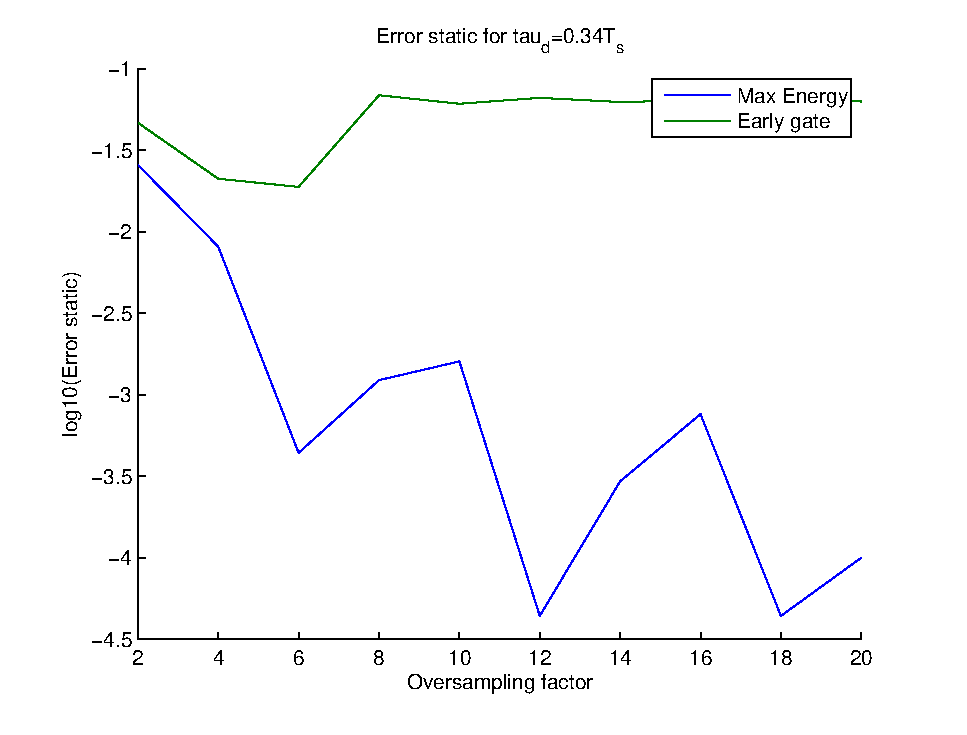
\includegraphics[width = 0.47 \textwidth]{err1.eps} &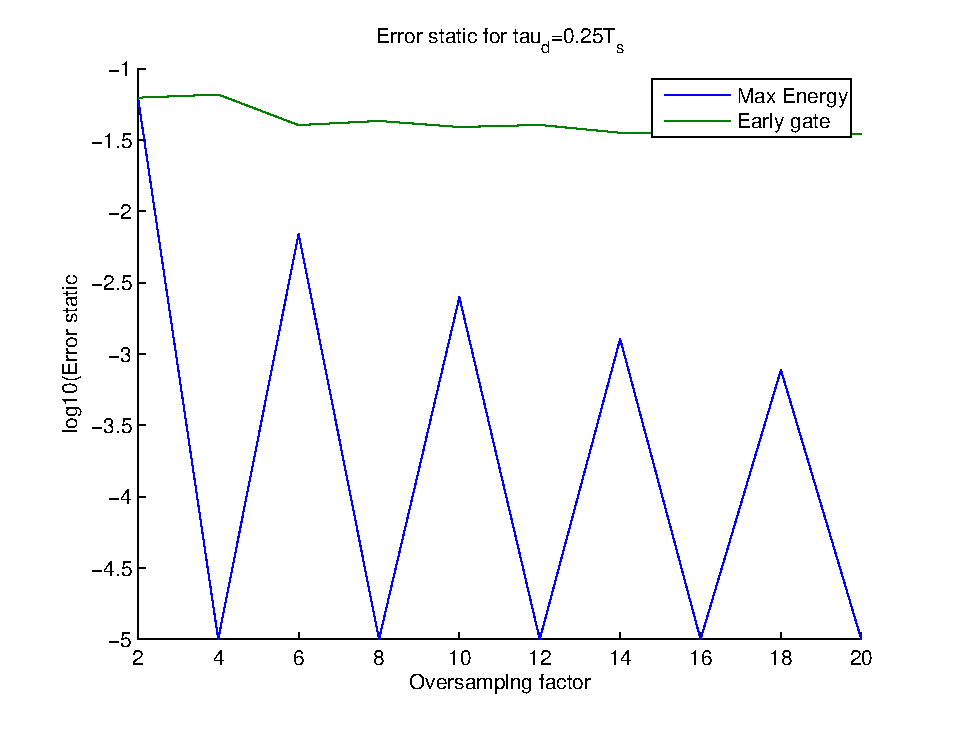
\includegraphics[width= 0.47 \textwidth]{err2.eps}
			\end{tabular}
		\end{figure}
		\end{frame}

		\begin{frame}{Error static}
			The shape of error static for direct maximization is due to the delay and the oversampling factor.
			\begin{figure}[h!]
				\center
				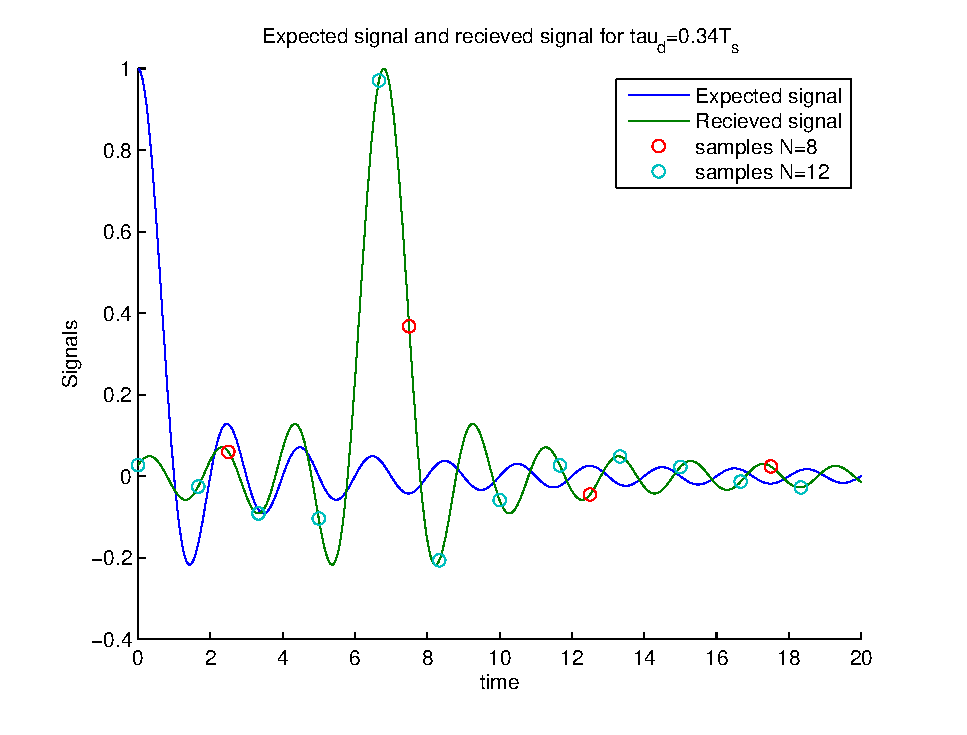
\includegraphics[width = \textwidth]{exp.eps}
			\end{figure}
		\end{frame}
	\subsubsection{Constellations}
	    \begin{frame}{Constellations}
	        \begin{figure}[h!]
	            \centering  
	            \begin{subfigure}[b]{0.3 \textwidth}
	                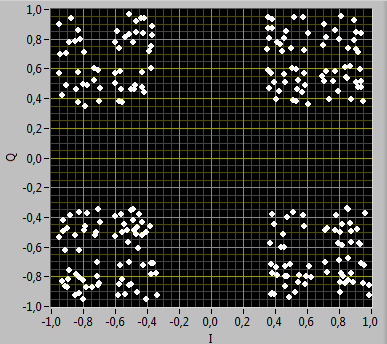
\includegraphics[width=\textwidth]{dir_2.PNG}
	                \caption{M = 2}\label{fig:2}
	            \end{subfigure}
	            ~	           
	            \begin{subfigure}[b]{0.3 \textwidth}
	           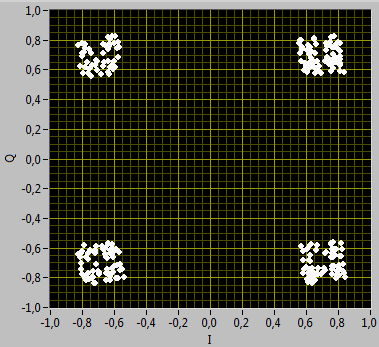
\includegraphics[width=\textwidth]{dir_4.PNG}
	                \caption{M = 4}\label{fig:4}
	            \end{subfigure}
	            
	            \begin{subfigure}[b]{0.3 \textwidth}
	                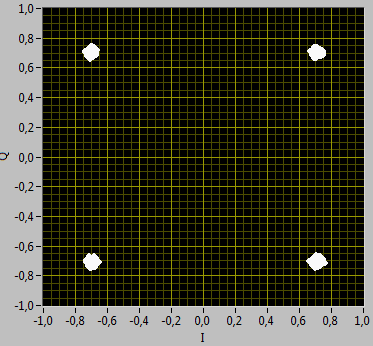
\includegraphics[width=\textwidth]{dir_10.PNG}
	                \caption{M = 10}\label{fig:10}
	            \end{subfigure}
	            ~	           
	            \begin{subfigure}[b]{0.3 \textwidth}
	           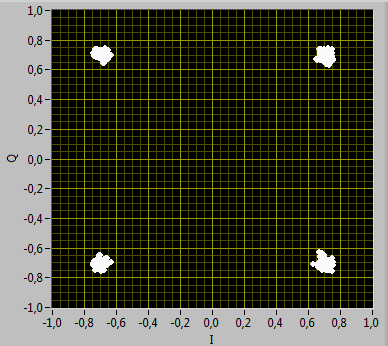
\includegraphics[width=\textwidth]{dir_20.PNG}
	                \caption{M = 20}\label{fig:20}
	            \end{subfigure}
	            \caption{Constellation for direct maximization}\label{fig:const}
	        \end{figure}
	    \end{frame}
	    
\section{Channel Estimation and Equalization}
 \begin{frame}{Channel estimation and equalization}
    Channel distortion ($h(t) \neq \delta (t)$) so received signal suffers from ISI :
    \begin{equation}
        y[n] = h[0]s[n] + \sum_{m \neq n} s[m]h[n-m] +v[n]
    \end{equation}
    
    \begin{itemize}
    \item Goal : reduce effect of channel (apply "inverse filter") = \textit{equalization}.
    \item Equalization needs the channel response before = channel \textit{estimation}.
    \end{itemize}
    
    
    Use a \textit{training sequence} to estimate the channel.\\
    Both methods use a \textit{least-squares approximation} method : expensive!
    
    \end{frame}
    
    
\begin{frame}{Direct least-squares equalization}
   \textit{Direct method} : apply channel estimation and equalization at once! Only 1 LLS.
   
   \begin{equation}
        \sum_{l=0}^{L_f} f[l] y[n + n_d - l] = t[n] \; \; , \; \; n = 0 ... N_t
   \end{equation}
   
   Estimate filter parameters $f[0]...f[L_f]$ by creating a filter that matches training sequence $t$ from the received signal $y$. 
   
   Note :
   \begin{itemize}
    \item $n_d$ = filter delay
    \item $L_f$ = filter length
    \end{itemize}
    
\end{frame}
    

\begin{frame}{Simulation : influence of channel length}
    Increasing $L_f$ from 1 to 6 (better estimations)
    \begin{figure}[h]
        \centering
        \begin{tabular}{ccc}
            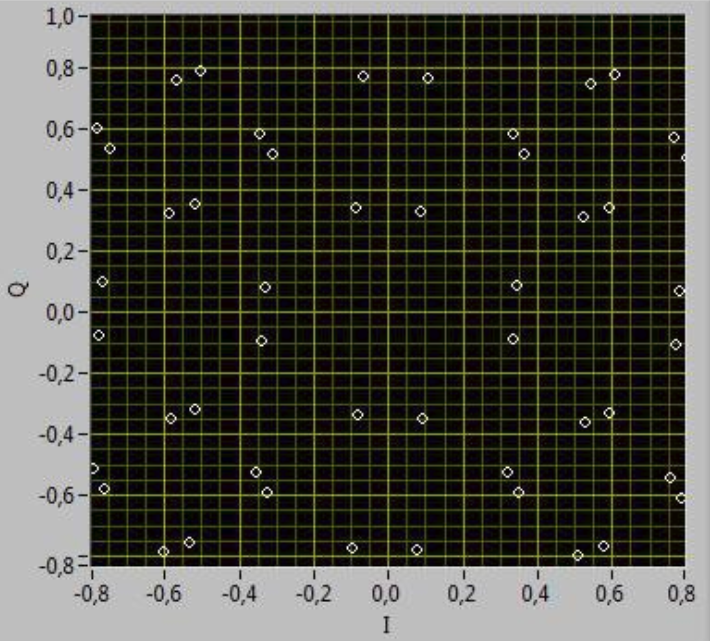
\includegraphics[width= 0.3 \textwidth]{eq1.png} & 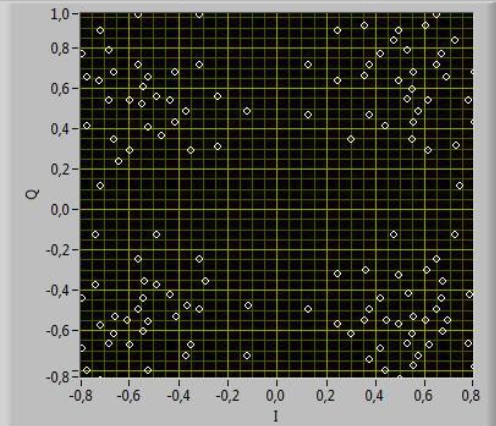
\includegraphics[width= 0.3 \textwidth]{eq2.png} & 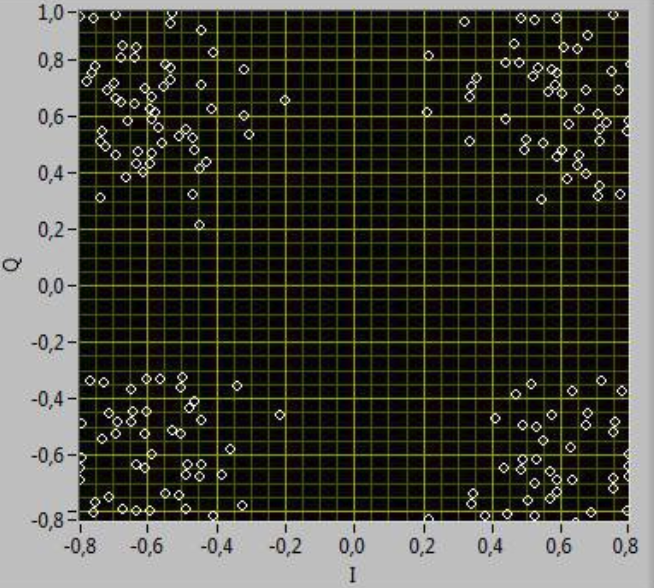
\includegraphics[width= 0.3 \textwidth]{eq3.png} \\
        \end{tabular}
    \end{figure}
    \begin{figure}[h]
        \centering
        \begin{tabular}{ccc}
            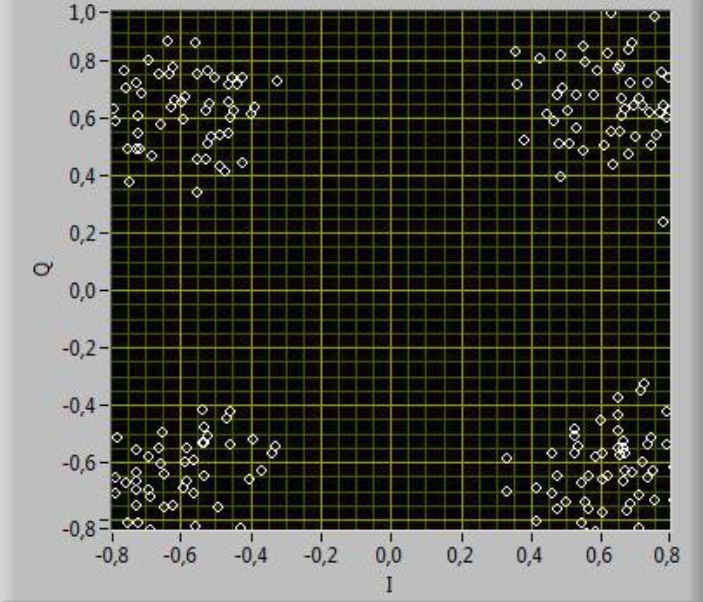
\includegraphics[width= 0.3 \textwidth]{eq4.png} & 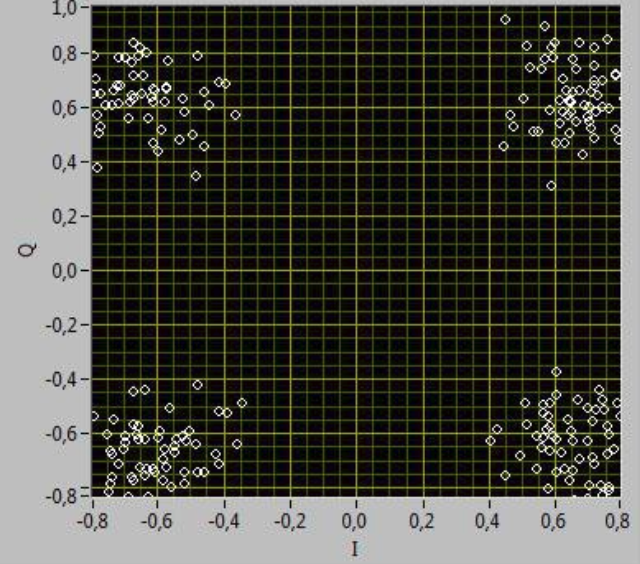
\includegraphics[width= 0.3 \textwidth]{eq5.png} & 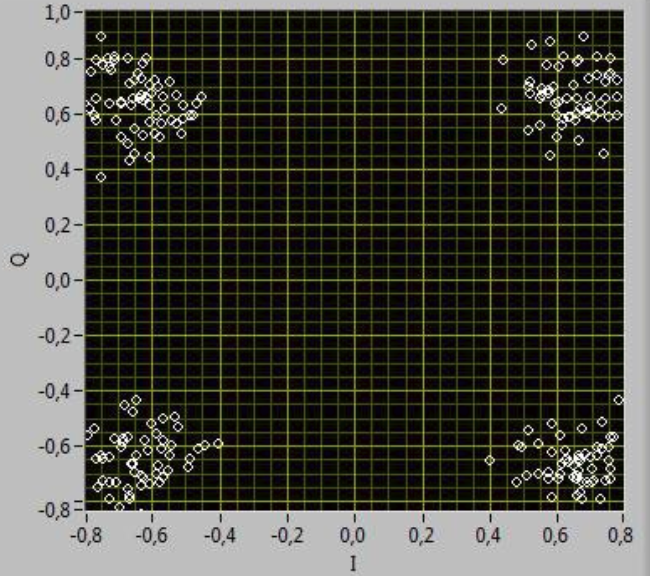
\includegraphics[width= 0.3 \textwidth]{eq6.png} \\
        \end{tabular}
    \end{figure}
\end{frame}

\begin{frame}{Simulation : influence of noise}
Noise on the training sequence corrupts the equalizer and propagates to all symbols! 

\begin{figure}[h]
        \centering
        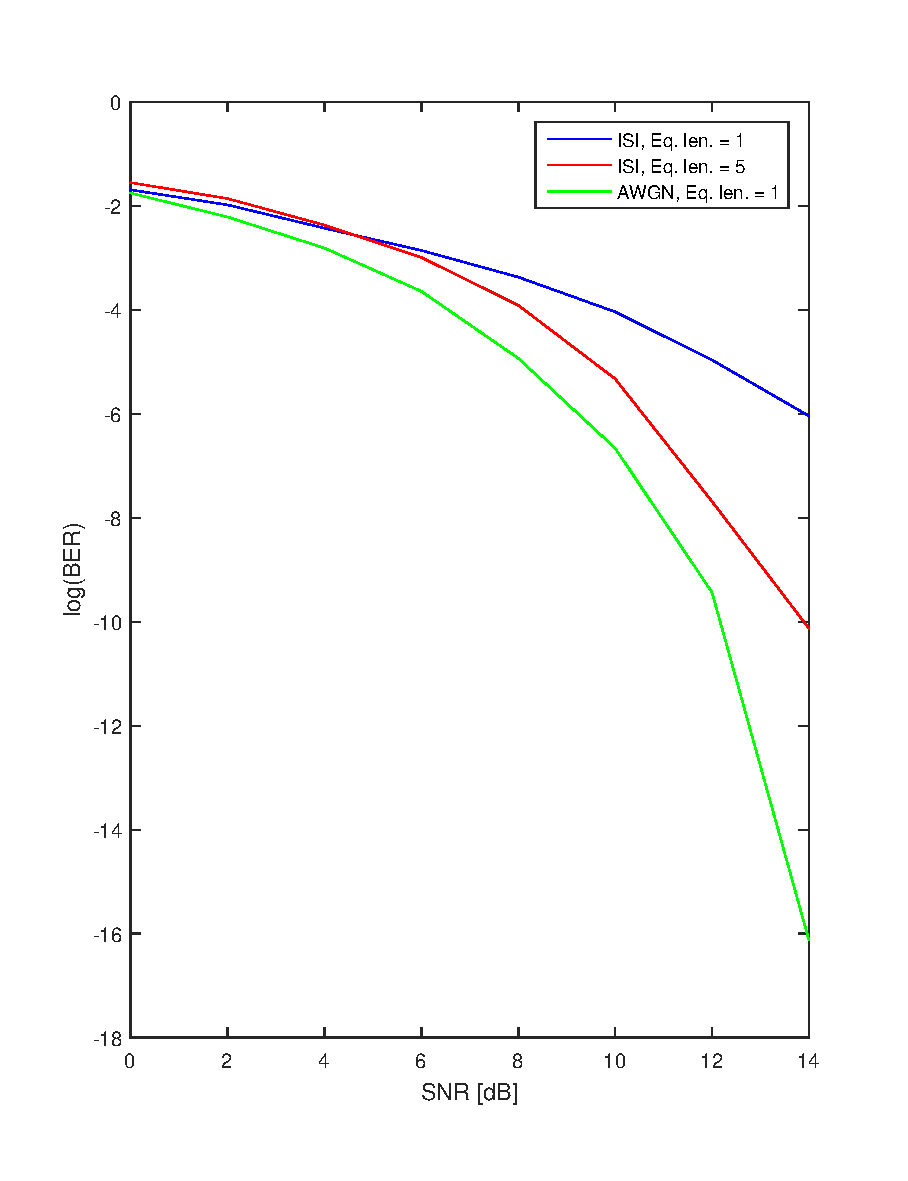
\includegraphics[scale = 0.4]{SNR1} 
            
    \end{figure}

\end{frame}

\begin{frame}{Experiment : effect of channel}
No equalization! Constellation shifted + scaled.


\begin{figure}[h!]
    \centering
    \begin{tabular}{cc}
     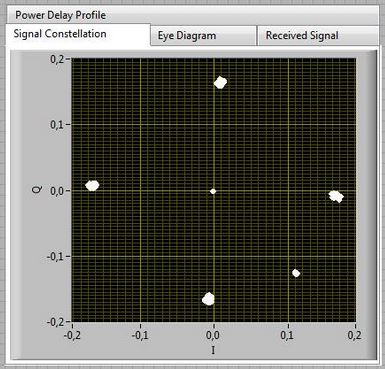
\includegraphics[scale = 0.45]{con1} & 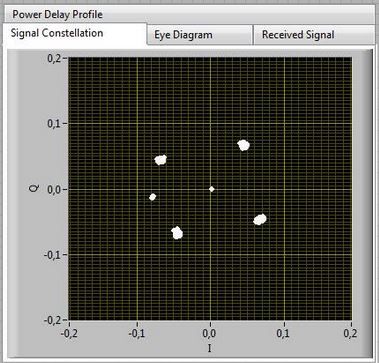
\includegraphics[scale = 0.45]{con2}\\
     & 
    \end{tabular}
    
    \caption{Received constellation without equalizer.}
    \label{con1}
\end{figure}



\end{frame}


\end{document}
